\chapter{Implementacija i korisničko sučelje}
		
		
		\section{Korištene tehnologije i alati}
		
			Tim je koristio \underline{WhatsApp}.\footnote[1]{https://www.whatsapp.com/} i \underline{Notion}.\footnote[2]{https://www.notion.so/} za komunikaciju unutar tima. Za izradu UML dijagrama korišten je \underline{Astah Professional}.\footnote[3]{https://astah.net/products/astah-professional/}, dok je za upravljanje izvornim kodom odabran \underline{Git}.\footnote[4]{https://git-scm.com/}. Udaljeni repozitorij projekta dostupan je na web platformi \underline{GitHub}.\footnote[5]{https://github.com/}.
			
			Kao razvojna okruženja korišteni su \underline{Visual Studio Code}.\footnote[6]{https://code.visualstudio.com/} i \underline{IntelliJ IDEA}.\footnote[7]{https://www.jetbrains.com/idea/}. Visual Studio Code je jednostavan uređivač koda s podrškom za razvojne operacije poput debugiranja, pokretanja zadataka i kontrolu verzija od tvrtke Microsoft, dok je IntelliJ popularno razvojno okruženje (IDE) razvijeno od strane tvrtke JetBrains. Namijenjeno je prvenstveno za rad s Java programskim jezikom.
			
			Aplikacija je napisana koristeći radni okvir \underline{Spring Boot}.\footnote[8]{https://spring.io/projects/spring-boot/} i jezik \underline{Java}.\footnote[9]{https://www.java.com/en/} za izradu backenda te \underline{React}.\footnote[10]{https://react.dev/} i jezik \underline{JavaScript}.\footnote[11]{https://www.javascript.com/} za izradu frontenda. React je besplatna i open-source JavaScript biblioteka za izgradnju korisničkih sučelja temeljenih na komponentama. Održava je Meta i zajednica pojedinačnih razvijatelja te tvrtki. Radni okvir Spring Boot je otvoreni, mikroservisni Java web okvir koji nudi Spring. Razvijen je kako bi pojednostavio proces izrade, konfiguracije i razmještanja Java aplikacija. 
			
			Baza podataka se nalazi na posluzitelju u oblaku \underline{Render}.\footnote[12]{https://render.com/}.
			
			
			\eject 
		
	
		\section{Ispitivanje programskog rješenja}
			\section{Ispitivanje komponenti}
			Napisati kratki opis sto se koristilo i kako za testove(JUnit 5 za unit testove)...
			
			\subsection{Ispitivanje funkcije emailRegexCheck:}
			Provjerava se funkcionalnost metode \textit{emailRegexCheck} u \textit{AuthenticationServiceJpa servisu} koja služi za provjeru ispravnog formata maila.
			
			\textbf{emailRegexCheckValidEmailReturnsTrue:}
			\begin{itemize}
				\item U funkciju se šalje mail ispravnog formata.
				\item Očekuje se da funkcija vraća true.
			\end{itemize}
			\begin{lstlisting}
			@Test
			void emailRegexCheck_ValidEmail_ReturnsTrue() {
				String validEmail = "test@example.com";
				boolean result = authenticationServiceJpa.emailRegexCheck(validEmail);
				assertTrue(result);
			}
			\end{lstlisting}
			
			\textbf{testEmailRegexCheckInvalidEmail:}
			\begin{itemize}
				\item U funkciju se šalje mail neispravnog formata.
				\item Očekuje se da funkcija vraća false.
			\end{itemize}
			\begin{lstlisting}
				@Test
				public void testEmailRegexCheckInvalidEmail() {
					String invalidEmail = "invalidemail";
					boolean isValid = authenticationServiceJpa.emailRegexCheck(invalidEmail);
					assertFalse(isValid);
				}
			\end{lstlisting}
			
			\textbf{testEmailRegexCheckInvalidEmailEdgeCase:}
			\begin{itemize}
				\item U funkciju se šalje mail neispravnog formata.
				\item Očekuje se da funkcija vraća false.
			\end{itemize}
			\begin{lstlisting}
				@Test
				public void testEmailRegexCheckInvalidEmail_EdgeCase() {
					String invalidEmail = "@.";
					boolean isValid = authenticationServiceJpa.emailRegexCheck(invalidEmail);
					assertFalse(isValid);
				}
			\end{lstlisting}
			\begin{figure}[H]
				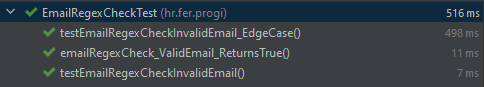
\includegraphics[scale=1]{slike/emailRegexTest.png} 
				\centering
				\caption{Rezultati ispitivanja}
				\label{fig:promjene}
			\end{figure}
			
			
			\subsection{Ispitivanje funkcije checkActionDto:}
			Provjerava se funkcionalnost metode \textit{checkActionDto} u \textit{researcherServiceJpa servisu} koja služi za provjeru ispravnosti podataka unutar \textit{ActionDto} objekta.
			
			\textbf{testCheckActionDtoValid:}
			\begin{itemize}
				\item U funkciju se šalje objekt \textit{ActionDto} s ispravnim podacima.
				\item Očekuje se da neće doći do bacanja iznimke.
			\end{itemize}
			\begin{lstlisting}
				@Test
				public void testCheckActionDtoValid() {
					ActionDto validActionDto = new ActionDto(1L, "ActionName", "ActionType", "LocationName");
					assertDoesNotThrow(() -> researcherServiceJpa.checkActionDto(validActionDto));
				}
			\end{lstlisting}
			
			\textbf{testCheckActionDtoInvalidNull:}
			\begin{itemize}
				\item U funkciju se šalje objekt \textit{ActionDto} s neispravnim podacima (\textit{actionName} postavljen na \textit{null}).
				\item Očekuje se da će doći do bacanja iznimke.
			\end{itemize}
			\begin{lstlisting}
				@Test
				public void testCheckActionDtoInvalidNull() {
					ActionDto invalidActionDto = new ActionDto(null, null, "ActionType", "LocationName");
					assertThrows(IllegalArgumentException.class, () -> researcherServiceJpa.checkActionDto(invalidActionDto));
				}
			\end{lstlisting}
			
			\textbf{testCheckActionDtoInvalidEmpty:}
			\begin{itemize}
				\item U funkciju se šalje objekt \textit{ActionDto} s neispravnim podacima (\textit{actionName} postavljen na \textit{""}).
				\item Očekuje se da će doći do bacanja iznimke.
			\end{itemize}
			\begin{lstlisting}
				@Test
				public void testCheckActionDtoInvalidEmpty() {
					ActionDto invalidActionDto = new ActionDto(1L, "", "ActionType", "LocationName");
					assertThrows(IllegalArgumentException.class, () -> researcherServiceJpa.checkActionDto(invalidActionDto));
				}
			\end{lstlisting}
			
			\textbf{testCheckActionDtoInvalidWhitespace:}
			\begin{itemize}
				\item U funkciju se šalje objekt \textit{ActionDto} s neispravnim podacima (\textit{actionName} postavljen na \textit{" ActionName"}).
				\item Očekuje se da će doći do bacanja iznimke.
			\end{itemize}
			\begin{lstlisting}
				@Test
				public void testCheckActionDtoInvalidWhitespace() {
					ActionDto invalidActionDto = new ActionDto(1L, " ActionName", "ActionType", "LocationName");
					assertThrows(IllegalArgumentException.class, () -> researcherServiceJpa.checkActionDto(invalidActionDto));
				}
			\end{lstlisting}
			
			\begin{figure}[H]
				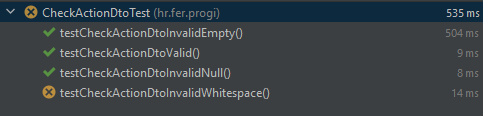
\includegraphics[scale=1]{slike/checkActionDtoTest.png} 
				\centering
				\caption{Rezultati ispitivanja}
				\label{fig:promjene}
			\end{figure}
			
			
			\subsection{Ispitivanje funkcije checkTaskDto:}
			Provjerava se funkcionalnost metode \textit{checkTaskDto} u \textit{taskServiceJpa servisu} koja služi za provjeru ispravnosti podataka unutar \textit{TaskDto} objekta.
			
			\textbf{testCheckTaskDtoValid:}
			\begin{itemize}
				\item U funkciju se šalje objekt \textit{TaskDto} s ispravnim podacima.
				\item Očekuje se da neće doći do bacanja iznimke.
			\end{itemize}
			\begin{lstlisting}
				@Test
				void testCheckTaskDtoValid() {
					TaskDto validTaskDto = new TaskDto(1L, 1L, new RouteWaypoints(), "TaskToDo", "TaskComment");
					assertDoesNotThrow(() -> taskServiceJpa.checkTaskDto(validTaskDto));
				}
			\end{lstlisting}
			
			\textbf{testCheckTaskDtoInvalidNull:}
			\begin{itemize}
				\item U funkciju se šalje objekt \textit{TaskDto} s neispravnim podacima (\textit{searcherId} postavljen na \textit{null}).
				\item Očekuje se da će doći do bacanja iznimke.
			\end{itemize}
			\begin{lstlisting}
				@Test
				public void testCheckActionDtoInvalidNull() {
					ActionDto invalidActionDto = new ActionDto(null, null, "ActionType", "LocationName");
					assertThrows(IllegalArgumentException.class, () -> researcherServiceJpa.checkActionDto(invalidActionDto));
				}
			\end{lstlisting}
			
			\textbf{testCheckTaskDtoInvalidEmpty:}
			\begin{itemize}
				\item U funkciju se šalje objekt \textit{TaskDto} s neispravnim podacima (\textit{taskToDo} postavljen na \textit{""}).
				\item Očekuje se da će doći do bacanja iznimke.
			\end{itemize}
			\begin{lstlisting}
				@Test
				void testCheckTaskDtoInvalidEmpty() {
					TaskDto invalidTaskDtoEmpty = new TaskDto(null, 1L, new RouteWaypoints(), "TaskComment", "");
					assertThrows(IllegalArgumentException.class, () -> taskServiceJpa.checkTaskDto(invalidTaskDtoEmpty));
				}
			\end{lstlisting}
			
			\textbf{testCheckTaskDtoInvalidWhitespace:}
			\begin{itemize}
				\item U funkciju se šalje objekt \textit{TaskDto} s neispravnim podacima (\textit{taskToDo} postavljen na \textit{"  TaskToDo"}).
				\item Očekuje se da će doći do bacanja iznimke.
			\end{itemize}
			\begin{lstlisting}
				@Test
				void testCheckTaskDtoInvalidWhitespace() {
					TaskDto invalidTaskDtoWhitespace = new TaskDto(null, 1L, new RouteWaypoints(), "TaskComment", "  TaskToDo");
					assertThrows(IllegalArgumentException.class, () -> taskServiceJpa.checkTaskDto(invalidTaskDtoWhitespace));
				}
			\end{lstlisting}
			
			\begin{figure}[H]
				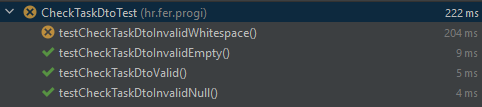
\includegraphics[scale=1]{slike/checkTaskDtoTest.png} 
				\centering
				\caption{Rezultati ispitivanja}
				\label{fig:promjene}
			\end{figure}
			
			
			\section{Ispitivanje sustava}
			
			
			Sustav smo detaljno testirali primjenom Selenium WebDriver dodatka unutar JUnit testova. Proveli smo dva ključna ispitivanja kako bismo osigurali funkcionalnost sustava: jedno je bilo usmjereno na proces prijave korisnika, dok je drugo obuhvatilo postupak registracije.
			
			\subsection{Ispitivanje Prijave Korisnika:}
			\textbf{testLoginValidCreds:}
			\begin{itemize}
				\item Unose se ispravne korisničke akreditacije (valjana e-mail adresa i lozinka).
				\item Provjerava se preusmjeravanje nakon prijave.
				\item Očekuje se da je korisnik uspješno preusmjeren na "dashboard".
			\end{itemize}
			\begin{lstlisting}
			@Test
			public void testLogin_ValidCreds(){
				ChromeOptions options = new ChromeOptions();
				options.addArguments("--remote-allow-origins=*");
				WebDriver driver = new ChromeDriver(options);
				driver.manage().timeouts().implicitlyWait(10, TimeUnit.SECONDS);
				driver.get("https://wildtrack-fe.onrender.com/login");
				
				WebElement element = driver.findElement(By.name("email"));
				element.sendKeys("admin@wildtrack.com");
				element = driver.findElement(By.name("password"));
				element.sendKeys("admin123");
				driver.findElement(By.cssSelector(".login-button")).click();
				
				try {
					Thread.sleep(5000);
				} catch (InterruptedException e) {
					e.printStackTrace();
				}
				String redirURL = driver.getCurrentUrl();
				boolean compRes = redirURL.contains("dashboard");
				
				assertEquals(compRes, true);
				
				driver.quit();
			}
			\end{lstlisting}
			
			\textbf{testLoginInValidCreds:}
			\begin{itemize}
				\item Unose se nevaljane korisničke akreditacije (neispravna e-mail adresa i lozinka).
				\item Provjerava se preusmjeravanje nakon pokušaja prijave.
				\item Očekuje se da korisnik nije preusmjeren na "dashboard".
			\end{itemize}
			\begin{lstlisting}
				@Test
				public void testLogin_InvalidCreds(){
					ChromeOptions options = new ChromeOptions();
					options.addArguments("--remote-allow-origins=*");
					WebDriver driver = new ChromeDriver(options);
					driver.manage().timeouts().implicitlyWait(10, TimeUnit.SECONDS);
					driver.get("https://wildtrack-fe.onrender.com/login");
					
					WebElement element = driver.findElement(By.name("email"));
					element.sendKeys("invalid");
					element = driver.findElement(By.name("password"));
					element.sendKeys("invalid");
					driver.findElement(By.cssSelector(".login-button")).click();
					
					String redirURL = driver.getCurrentUrl();
					boolean compRes = redirURL.contains("dashboard");
					
					assertEquals(compRes, false);
					
					driver.quit();
				}
			\end{lstlisting}
			
			\textbf{testLoginEmptyEmail:}
			\begin{itemize}
				\item Ostavlja se polje za e-mail prazno.
				\item Postavlja se lozinka na neku vrijednost.
				\item Provjerava se preusmjeravanje nakon pokušaja prijave.
				\item Očekuje se da korisnik nije preusmjeren na "dashboard".
			\end{itemize}
			\begin{lstlisting}
				@Test
				public void testLogin_emptyEmail() {
					ChromeOptions options = new ChromeOptions();
					options.addArguments("--remote-allow-origins=*");
					WebDriver driver = new ChromeDriver(options);
					driver.manage().timeouts().implicitlyWait(10, TimeUnit.SECONDS);
					driver.get("https://wildtrack-fe.onrender.com/login");

					WebElement emailElement = driver.findElement(By.name("email"));
					emailElement.sendKeys("");
					
					WebElement passwordElement = driver.findElement(By.name("password"));
					passwordElement.sendKeys("somePassword");
					
					driver.findElement(By.cssSelector(".login-button")).click();
					
					String redirURL = driver.getCurrentUrl();
					boolean compRes = redirURL.contains("dashboard");
					
					assertEquals(compRes, false);
					
					driver.quit();
				}
			\end{lstlisting}
			
			\begin{figure}[H]
				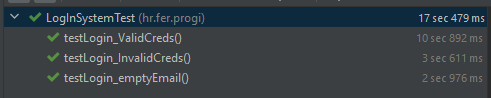
\includegraphics[scale=1]{slike/loginTests.png} 
				\centering
				\caption{Rezultati ispitivanja}
				\label{fig:promjene}
			\end{figure}
			
			Drugo ispitivanje bilo je usmjereno na proces registracije novog korisnika. Kroz Selenium WebDriver testove, simulirali smo korisničko sučelje kako bismo provjerili ispravnost postupka registracije. Cilj je bio osigurati da sustav adekvatno obrađuje unos novih korisničkih podataka te da novi korisnik bude uspješno registriran u sustavu.
			
			\textit{Ključne Točke Ispitivanja:}
			\begin{itemize}
				\item Popunjavanje obrasca za registraciju s valjanim podacima.
				\item Klik na gumb za registraciju.
				\item Provjera uspješne registracije i ispravnosti prelaska na stranicu nakon registracije.
			\end{itemize}
			
			\subsection{Ispitivanje Registracije:}
			\textbf{testRegistrationInvalidCreds:}
			\begin{itemize}
				\item Unosi se email u neispravnom formatu.
				\item Provjerava se ispisan tekst na stranici.
				\item Očekuje se je da je na stranici ispisan tekst \textit{email not valid}.
			\end{itemize}
			\begin{lstlisting}
				@Test
				public void testRegistration_InvalidCreds(){
					ChromeOptions options = new ChromeOptions();
					options.addArguments("--remote-allow-origins=*");
					WebDriver driver = new ChromeDriver(options);
					driver.manage().timeouts().implicitlyWait(10, TimeUnit.SECONDS);
					driver.get("https://wildtrack-fe.onrender.com/register");
					
					WebElement firstNameInput = driver.findElement(By.id("register-firstName"));
					firstNameInput.sendKeys("test");
					
					WebElement lastNameInput = driver.findElement(By.id("register-lastName"));
					lastNameInput.sendKeys("test");
					
					WebElement usernameInput = driver.findElement(By.id("register-username"));
					usernameInput.sendKeys("test");
					
					WebElement emailInput = driver.findElement(By.id("register-email"));
					emailInput.sendKeys("test");
					
					WebElement passwordInput = driver.findElement(By.id("register-password"));
					passwordInput.sendKeys("test");
					
					WebElement tragacRadioButton = driver.findElement(By.id("register-searcher"));
					tragacRadioButton.click();
					
					WebElement fileInput = driver.findElement(By.id("photo-upload"));
					fileInput.sendKeys("D:\\FER-predmeti\\zoolanders\\zoolanders\\be\\src
					\\test\\resources\\profile.jpg");
					
					WebElement registerButton = driver.findElement(By.cssSelector(".register-button"));
					registerButton.click();
					
					try {
						Thread.sleep(10000);
					} catch (InterruptedException e) {
						e.printStackTrace();
					}
					WebElement errorElement = driver.findElement(By.className("register-error"));
					String actualErrorText = errorElement.getText();
					String expectedErrorText = "email not valid";
					
					assertEquals(expectedErrorText, actualErrorText);
					
					driver.quit();
				}
			\end{lstlisting}
			
			\textbf{testRegistrationEmailAllReadyTaken:}
			\begin{itemize}
				\item Unose se korisnički podaci u ispravnom formatu.
				\item Provjerava se ispisan tekst na stranici.
				\item Očekuje se je da je na stranici ispisan tekst \textit{email already taken}.
			\end{itemize}
			\begin{lstlisting}
				@Test
				public void testRegistration_InvalidCreds(){
					ChromeOptions options = new ChromeOptions();
					options.addArguments("--remote-allow-origins=*");
					WebDriver driver = new ChromeDriver(options);
					driver.manage().timeouts().implicitlyWait(10, TimeUnit.SECONDS);
					driver.get("https://wildtrack-fe.onrender.com/register");
					
					WebElement firstNameInput = driver.findElement(By.id("register-firstName"));
					firstNameInput.sendKeys("test");
					
					WebElement lastNameInput = driver.findElement(By.id("register-lastName"));
					lastNameInput.sendKeys("test");
					
					WebElement usernameInput = driver.findElement(By.id("register-username"));
					usernameInput.sendKeys("test");
					
					WebElement emailInput = driver.findElement(By.id("register-email"));
					emailInput.sendKeys("test");
					
					WebElement passwordInput = driver.findElement(By.id("register-password"));
					passwordInput.sendKeys("test");
					
					WebElement tragacRadioButton = driver.findElement(By.id("register-searcher"));
					tragacRadioButton.click();
					
					WebElement fileInput = driver.findElement(By.id("photo-upload"));
					fileInput.sendKeys("D:\\FER-predmeti\\zoolanders\\zoolanders\\be\\src
					\\test\\resources\\profile.jpg");
					
					WebElement registerButton = driver.findElement(By.cssSelector(".register-button"));
					registerButton.click();
					
					try {
						Thread.sleep(10000);
					} catch (InterruptedException e) {
						e.printStackTrace();
					}
					WebElement errorElement = driver.findElement(By.className("register-error"));
					String actualErrorText = errorElement.getText();
					String expectedErrorText = "email not valid";
					
					assertEquals(expectedErrorText, actualErrorText);
					
					driver.quit();
				}
			\end{lstlisting}
			
			\textbf{testRegistrationValidCreds:}
			\begin{itemize}
				\item Unose se korisnički podaci u ispravnom formatu.
				\item Provjerava se ispisan tekst na stranici.
				\item Očekuje se je da je na stranici ispisan tekst \textit{Registracija uspješna!}.
			\end{itemize}
			\begin{lstlisting}
				@Test
				public void testRegistration_ValidCreds(){
					ChromeOptions options = new ChromeOptions();
					options.addArguments("--remote-allow-origins=*");
					WebDriver driver = new ChromeDriver(options);
					driver.manage().timeouts().implicitlyWait(10, TimeUnit.SECONDS);
					driver.get("https://wildtrack-fe.onrender.com/register");
					
					WebElement firstNameInput = driver.findElement(By.id("register-firstName"));
					firstNameInput.sendKeys("test");
					
					WebElement lastNameInput = driver.findElement(By.id("register-lastName"));
					lastNameInput.sendKeys("test");
					
					WebElement usernameInput = driver.findElement(By.id("register-username"));
					usernameInput.sendKeys("test");
					
					WebElement emailInput = driver.findElement(By.id("register-email"));
					emailInput.sendKeys("test1@test.com");
					
					WebElement passwordInput = driver.findElement(By.id("register-password"));
					passwordInput.sendKeys("test");
					
					WebElement tragacRadioButton = driver.findElement(By.id("register-searcher"));
					tragacRadioButton.click();
					
					WebElement fileInput = driver.findElement(By.id("photo-upload"));
					fileInput.sendKeys("D:\\FER-predmeti\\zoolanders\\zoolanders\\be\\src
					\\test\\resources\\profile.jpg");
					
					WebElement registerButton = driver.findElement(By.cssSelector(".register-button"));
					registerButton.click();
					
					try {
						Thread.sleep(10000);
					} catch (InterruptedException e) {
						e.printStackTrace();
					}
					WebElement errorElement = driver.findElement(By.className("register-success"));
					String actualText = errorElement.getText();
					String expectedText = "Registracija uspješna!";
					
					assertEquals(expectedText, actualText);
					
					driver.quit();
				}
			\end{lstlisting}
			
			\begin{figure}[H]
				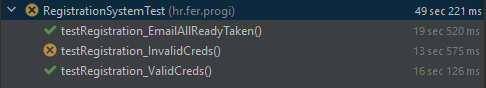
\includegraphics[scale=1]{slike/registrationTests.png} 
				\centering
				\caption{Rezultati ispitivanja}
				\label{fig:promjene}
			\end{figure}
			
			\eject 
		
		
		\section{Dijagram razmještaja}
			
			\textbf{\textit{dio 2. revizije}}
			
			 \textit{Potrebno je umetnuti \textbf{specifikacijski} dijagram razmještaja i opisati ga. Moguće je umjesto specifikacijskog dijagrama razmještaja umetnuti dijagram razmještaja instanci, pod uvjetom da taj dijagram bolje opisuje neki važniji dio sustava.}
			
			\eject 
		
		\section{Upute za puštanje u pogon}
		
			\textbf{\textit{dio 2. revizije}}\\
		
			 \textit{U ovom poglavlju potrebno je dati upute za puštanje u pogon (engl. deployment) ostvarene aplikacije. Na primjer, za web aplikacije, opisati postupak kojim se od izvornog kôda dolazi do potpuno postavljene baze podataka i poslužitelja koji odgovara na upite korisnika. Za mobilnu aplikaciju, postupak kojim se aplikacija izgradi, te postavi na neku od trgovina. Za stolnu (engl. desktop) aplikaciju, postupak kojim se aplikacija instalira na računalo. Ukoliko mobilne i stolne aplikacije komuniciraju s poslužiteljem i/ili bazom podataka, opisati i postupak njihovog postavljanja. Pri izradi uputa preporučuje se \textbf{naglasiti korake instalacije uporabom natuknica} te koristiti što je više moguće \textbf{slike ekrana} (engl. screenshots) kako bi upute bile jasne i jednostavne za slijediti.}
			
			
			 \textit{Dovršenu aplikaciju potrebno je pokrenuti na javno dostupnom poslužitelju. Studentima se preporuča korištenje neke od sljedećih besplatnih usluga: \href{https://aws.amazon.com/}{Amazon AWS}, \href{https://azure.microsoft.com/en-us/}{Microsoft Azure} ili \href{https://www.heroku.com/}{Heroku}. Mobilne aplikacije trebaju biti objavljene na F-Droid, Google Play ili Amazon App trgovini.}
			
			
			\eject 